% LaTeX2e Template by Stephen Iota (https://stepheniota.github.io/)
% last updated: Aug. 2018

% for papers
%\documentclass[aps,onecolumn,superscriptaddress]{revtex4-1}

% https://www-d0.fnal.gov/Run2Physics/WWW/templates/revtex4.pdf
% https://cdn.journals.aps.org/files/revtex/auguide4-1.pdf
% for revTeX4-1 class options

% for other
\documentclass[12pt]{article}
\usepackage[margin=2cm]{geometry}

%%%%%%%%%%%%%%%%
%%% Packages %%%
%%%%%%%%%%%%%%%%

\usepackage[utf8]{inputenc}
\usepackage{amsmath}
\usepackage{amssymb}
\usepackage{amsfonts} % to remove math font when typesetting equations
\usepackage{graphicx}
\usepackage{enumitem} % to change labels in enum/item
\usepackage[dvipsnames]{xcolor} % for colored links


% always put this at the end
\usepackage[
	colorlinks=true,
	citecolor=green!50!black,
	linkcolor=NavyBlue!75!black,
	urlcolor=green!50!black,
	hypertexnames=false]{hyperref} 

 
 %%%%%%%%%%%%%%%%%%
 %% New Commands %%
 %%%%%%%%%%%%%%%%%%
 
\newcommand{\email}[1]{\texttt{\href{mailto:#1}{#1}}}

\newcommand{\hint}[1]{\color{Blue}{#1}}
 
%----------------------------------------------------
%%%%%%%%%%%%%%%%%%
%% Front Matter %%
%%%%%%%%%%%%%%%%%%

%\pagenumbering{gobble} % no page numbers
\graphicspath{{figures/}} % set directory for figures

%%%%%%%%%%%%%
%%% Title %%%
%%%%%%%%%%%%%
\begin{document}

\begin{center}

\Large{\textsc{Worksheet 2a}: \textbf{Charge Distributions}}

\end{center}

\vspace{.5mm}

%%%%%%%%%%
%% INFO %%
%%%%%%%%%%

\begin{tabular}{rl}
\textsc{SI Leader}:
&
Stephen Iota (\email{siota001@ucr.edu})
\\
\textsc{Course}:
&
Physics 40C (Fall 2018); Dr.~Laura Sales
\\
\textsc{Date}:
&
October 9, 2018
\end{tabular}

%%%%%%%%%%%%%%
%% PROBLEMS %%
%%%%%%%%%%%%%%

\subsubsection*{README}

``\textit{How do I even start this problem?!}''\\
1) Take a deep breath
2) carefully read the question
3) draw and label figure and axes
4) identify unknown and knowns
5) write down relevant concepts and equations and 
6) crunch the numbers!


\section{Conceptual Questions}

\begin{enumerate}[label=(\alph*)]
\item Give examples of symmetric shapes and non-symmetric shapes.
\item When is the dipole approximation valid?
\item Describe the dynamics of a dipole placed in a \textbf{uniform} electric field.
\begin{itemize}
	\item Does it experience a force?
	\item Does it move? If so, how?
\end{itemize}
\item At the dot, in what direction does the electric field point?
 
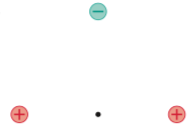
\includegraphics[width=.2\linewidth]{W2a_Fig1.png}
\item What are ways to increase the magnitude of the electric field at the dot?

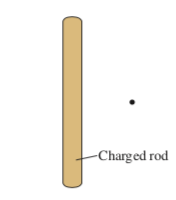
\includegraphics[width=.2\linewidth]{W2a_Fig2}
\item Draw the electric field lines for the positively charged rod above.
\item How much faster does the $\vec{E}$ field of a point charge decay compared to the $\vec{E}$ field of a charged-thin wire?
\end{enumerate}

\section{The Electric Field of a Continuous Distribution}

\begin{enumerate}[label=(\alph*)]
	\item The electric field strength $10.0$ cm away from a very long charged wire\footnote{\label{text}Look in text/notes to find relevant $\vec{E}$ field equation.} is $2000$ N/C. What is the electric field strength $5.0$ cm from the wire?
	
	\item The electric field strength $2.0$ cm from the surface of a $10$-cm-diameter metal ball\footnote{See footnote 1.} is $50,000$ N/C. What is the total  charge $Q$ (in nC) on the metal ball?
\end{enumerate}



\section{Thin Charged Wire}

No notes or textbook this time! 
Show that the electric field $\vec{E}$ at point $p$ a distance $r$ above an infinite wire with total charge $Q$ is: 
$$\vec{E}(p) = \frac{1}{4\pi\epsilon}\int_{-\frac{L}{2}}^ \frac{L}{2} \! \mathrm{d}x \ \frac{\lambda x}{(r^2 + x^2)^\frac{3}{2}}  \ \hat{y}$$

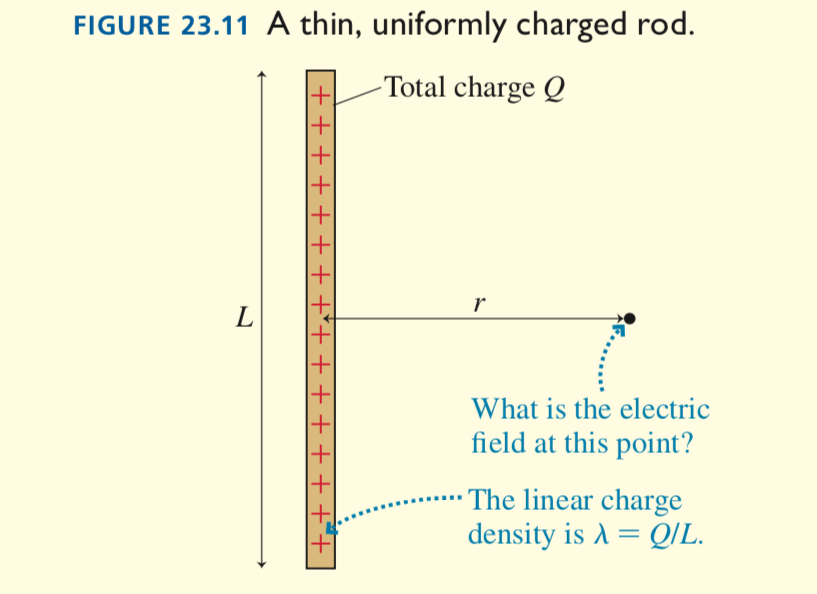
\includegraphics[width=.4\linewidth]{W2a_fig3.png}

\hint{\texttt{Hint 1}: See problem 1(a)}

\hint{\texttt{Hint 2}: Use that one theorem by that one greek guy... Pythagoras!}

\hint{\texttt{Hint 3}: There's a $\cos{\theta}$ in there at some point...}

\hint{\texttt{Hint 4}: No more hints!}{

\end{document}